\documentclass[a4paper, 11pt]{article}

% Packages
\usepackage[margin=2cm, bottom=0.6cm]{geometry}
\usepackage{graphicx}
\usepackage{caption}
\usepackage{tikz}
\usepackage{enumitem}
\usepackage{fontawesome}
\usepackage{calligra}
\usepackage{xcolor}
\usepackage{hyperref}
\hypersetup{
    colorlinks=false,
    hidelinks
}

% Personal Data
\newcommand{\firstname}{Alessandro}
\newcommand{\lastname}{Azzani}
\newcommand{\nationality}{Italian}
\newcommand{\address}{Cäsar-Ritz-Strasse 5, Zurich, Switzerland}
\newcommand{\birth}{22 February 2000}
\newcommand{\phone}{\href{tel:+393881012096}{+39~3881012096}}
\newcommand{\email}{\href{mailto:aazzani@student.ethz.ch}{aazzani@student.ethz.ch}}
\newcommand{\github}{\href{https://github.com/alessandroazzani}{alessandroazzani}}
\newcommand{\linkedin}{\href{https://www.linkedin.com/in/alessandro-azzani-3506b6234}{Alessandro Azzani}}

% Colors
\definecolor{ETHBlue}{RGB}{77, 125, 191}
\newcommand{\mycolor}{ETHBlue}    %General color
\definecolor{persdata}{RGB}{128, 128, 128}
\definecolor{colorlink}{RGB}{170, 170, 170}
\definecolor{colorsubtitle}{RGB}{70, 70, 70}
\definecolor{ETHlightblu}{RGB}{122, 157, 207}

%Setup itemize
\newcommand{\bluecircle}{\textcolor{\mycolor}{\textbullet}}
\newenvironment{noindentitem}[1]{
    \begin{itemize}[itemsep = -4pt, topsep = -1pt, label=\textcolor{\mycolor}{\textopenbullet}, leftmargin=1.2em]
        #1
}{
    \end{itemize}
}
\newenvironment{indentitem}[1]{
    \begin{itemize}[itemsep = -4pt, topsep = -1pt, label=\bluecircle]
        #1
}{
    \end{itemize}
}

% Setup sizes and widths
\pagestyle{empty}
\newcommand{\now}{Present}
\newcommand{\leftcolumwidth}{0.25}
\newcommand{\rightcolumwidth}{0.65}
\newcommand{\intersectionsep}{\vspace{2em}}
\newcommand{\intrasectionsep}{\vspace{0.6em}}
\newcommand{\sectionlinethickness}{2pt}
\newlength{\midl}
\setlength{\midl}{\dimexpr(\textwidth - \leftcolumwidth\textwidth - \rightcolumwidth\textwidth - 0.05\textwidth)\relax}
\setlength{\labelsep}{.5em}
\setlength{\leftmargini}{2em}
\addtolength{\labelwidth}{0em}

% Define CV commands
\newcommand{\cvsection}[1]{
    \setlength\topsep{0pt}%
    \begin{minipage}[c]{\leftcolumwidth\textwidth}%
        \raggedleft
        \textcolor{\mycolor}{\MakeUppercase{\bfseries \sffamily #1}}%
    \end{minipage}%
    \hspace{\midl}%
    \textcolor{\mycolor}{\noindent\rule[0em]{\rightcolumwidth\textwidth}{\sectionlinethickness}}%
    \vspace{-\baselineskip}%
    \intersectionsep%
}
\newcommand{\cvline}[2]{
    \setlength\topsep{0pt}%
    \begin{minipage}[t]{\leftcolumwidth\textwidth}%
        \raggedleft
        {#1}
    \end{minipage}%
    \hspace{\midl}%
    \begin{minipage}[c]{\rightcolumwidth\textwidth}
        {#2}
    \end{minipage}
}
\newcommand{\cventry}[3]{
    \cvline{#1}{#2}

    \cvline{\phantom{Void}}{#3}
}
\newcommand{\cventryright}[1]{
    \cvline{\phantom{Void}}{#1}
}
\newcommand{\cvpdf}[1]{
    \href{#1}{\textcolor{colorlink}{\faFilePdfO}}
}
\newcommand{\cvcode}[1]{
    \href{#1}{\textcolor{colorlink}{\faCode}}
}
\newcommand{\cvlink}[1]{
    \href{#1}{\textcolor{colorlink}{\faLink}}
}
\newcommand{\makeprivacy}{
    \vfill
    {
        \begin{center}
            \textcolor{gray}{\small I authorize the processing of personal data pursuant to Legislative Decree 196/2003}
        \end{center}
    }
}


% Document -------------------------------------------
\begin{document}
% Header -----------------------------------
% Picture
\begin{minipage}{0.28\textwidth}
    \begin{tikzpicture}
        \node [circle, minimum width=0.9\linewidth, draw, ultra thick, draw=\mycolor, path picture={\node at (path picture bounding box.center) {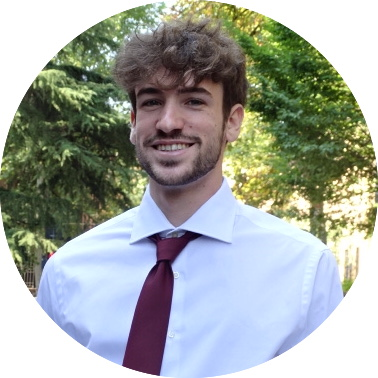
\includegraphics[width=0.9\linewidth]{photo_cv.jpg}};}] {};
    \end{tikzpicture}
\end{minipage}
\hfill
\begin{minipage}{0.65\textwidth}
    \vspace*{\fill}
    % First name and Last name
    {\Huge \bfseries \firstname\ \lastname} \\     % Different fonts: sffamily, bfseries, scshape, upshape
    \vspace{0.cm}

    % Personal information table
    \begin{tabular}{@{}cl@{}}
        \textcolor{persdata}{\faGlobe} & \textcolor{persdata}{\nationality} \\
        \textcolor{persdata}{\faCalendar} & \textcolor{persdata}{\birth} \\
        \textcolor{persdata}{\faMapMarker} & \textcolor{persdata}{\address} \\
        \textcolor{persdata}{\faPhone} & \textcolor{persdata}{\phone} \\
        \textcolor{persdata}{\faEnvelope} & \textcolor{persdata}{\email} \\
        \textcolor{persdata}{\faGithub} & \textcolor{persdata}{\github} \\
        \textcolor{persdata}{\faLinkedin} & \textcolor{persdata}{\linkedin} \\
    \end{tabular}
\end{minipage}
\vspace{0.7cm}

%Education
\cvsection{Education}

\cventry{\itshape Sep 2022 - \now}{
    {\bfseries \large ETH Zürich}
    \hfill
    {\upshape Zurich, Switzerland}}
    {\textcolor{colorsubtitle}{\slshape \bfseries Master's Degree in Physics}}

\intrasectionsep
\cventryright{
    \underline{Semester Thesis:}
    \begin{indentitem}
        \item {\scshape Title:} \emph{“Gluing Manifolds in the BV-BFV Formalism"}\cvpdf{https://drive.google.com/file/d/1cGkk3KFnYz9RpT1O9RomD194dyylY2_R/view?usp=share_link}
        \item {\scshape Supervisor:} Dr. Nima Moshayedi
        \item {\scshape Official supervisor:} Prof. Dr. Gian Michele Graf
    \end{indentitem}
}
\intersectionsep

\cventry{\itshape Sep 2019 - Jul 2022}{
    {\bfseries \large University of Bologna}
    \hfill
    {\upshape Bologna, Italy}}
    {\textcolor{colorsubtitle}{\slshape \bfseries Bachelor's Degree in Physics}}

\intrasectionsep
\cventryright{
    \underline{Final grade:} {$110 / 110$ cum laude}\cvpdf{https://drive.google.com/file/d/1CEhzsCPFQEI_VTm2NJPYABiaq-3fuA9z/view?usp=share_link}
    \intrasectionsep

    \underline{Thesis:}
    \begin{indentitem}
        \item {\scshape Title:} \emph{“Spectral Methods in Geometric Deep Learning"}\cvpdf{https://drive.google.com/file/d/1c7L6v-RiZEGCqzFQQPZbMFgASe07KFnD/view?usp=share_link}
        \item {\scshape Supervisor:} Prof. Dr. Rita Fioresi
    \end{indentitem}
}
\intersectionsep

\cventry{\itshape Sep 2014 - Jul 2019}{
    {\bfseries \large Liceo Scientifico “A. Tassoni"}
    \hfill
    {\upshape Modena, Italy}}
    {\textcolor{colorsubtitle}{\slshape \bfseries Highschool Diploma}}
\intrasectionsep

\cventryright{
    \underline{Final grade:} $100/100$\cvpdf{https://drive.google.com/file/d/1hp-SsgCZeJf3vNHCAivQV3V1a2u1ooJA/view?usp=share_link}
    \intrasectionsep

    \begin{noindentitem}
        \item Highschool with a focus on scientific subjects
    \end{noindentitem}
}

%Work Experience
\intersectionsep
\cvsection{Work Experience}

\cvline{\itshape 2019 - \now}{{\bfseries \large Private Tutor}
    \hfill
    {\upshape Modena, Italy / Online}}
\intrasectionsep

\cventryright{
    \begin{noindentitem}
        \item Tutoring highschool and undergraduate students on scientific subjects, e.g. mathematics, physics and chemistry
    \end{noindentitem}
}

% Conferences
\intersectionsep
\cvsection{Conferences}

\cvline{\itshape 25 - 28 Jul 2022}{{\bfseries \large School in Geometric Deep Learning}\cvpdf{https://drive.google.com/file/d/1YVXCChKXKbsBhStqj5RHf12GoFSJ7tnL/view?usp=share_link}
\hfill
{Pescara, Italy}}
\intrasectionsep

\cventryright{
    \begin{noindentitem}
        \item Intensive school focused on Geometric Deep Learning and its applications
        \item \underline{Speakers:} Prof. Micheal Bronstein, Christian Bodnar and Francesco Di Giovanni
    \end{noindentitem}
}

\newpage
% Extra Activities
\cvsection{Extra activities}

\cventry{
    \itshape Sep 2018 - Jul 2019
}{
    {\bfseries \large Vecchi-Tonelli Conservatory}
    \hfill
    {Modena, Italy}
}{
    \textcolor{colorsubtitle}{\bfseries \slshape Higher Institute of Musical Studies}
}

\intrasectionsep
\cventryright{
    \begin{noindentitem}
        \item Piano player in various bands and orchestras
        \item Started learning piano in 2008 with private lessons
    \end{noindentitem}
}

\intersectionsep
\cventry{
    \itshape Sep 2019 - Dec 2019
}{
    {\large \bfseries University-Hospital of Modena}
    \hfill
    {Modena, Italy}
}{
    \textcolor{colorsubtitle}{
        \slshape \bfseries Volunteering
    }
}

\intrasectionsep
\cventryright{
    \begin{noindentitem}
        \item Supportive role for nurses
        \item Helped patients in everyday tasks
    \end{noindentitem}
}

\intersectionsep
\cventry{
    \itshape Sep 2012 - Oct 2019
}{
    {\large \bfseries A.S. La Fratellanza 1874}
    \hfill
    {Modena, Italy}
}{
    \textcolor{colorsubtitle}{
        \slshape \bfseries Athletics
    }
}

\intrasectionsep
\cventryright{
    \begin{noindentitem}
        \item Specialized in high jump and pole jump
        \item Competed for regional leading athletics club
    \end{noindentitem}
}

% Languages
\intersectionsep
\cvsection{Languages}

\cventryright{
    \begin{tabular}{l l @{\hspace{1cm}} l}
        \textcolor{\mycolor}{\textbullet} \hspace{0.5mm} {\bfseries Italian:} & {\slshape Native} \\
        \textcolor{\mycolor}{\textbullet} \hspace{0.5mm} {\bfseries English:} & {\slshape Fluent} & IELTS certificate: C1\cvpdf{https://drive.google.com/file/d/1w0UrpZbEwPjNDb3oM7pGBj6oD0MPf8yx/view?usp=share_link} \\
        \textcolor{\mycolor}{\textbullet} \hspace{0.5mm} {\bfseries German:}  & {\slshape Basic } & ETH german course: A2
    \end{tabular}
}

% Digital skills
\intersectionsep
\cvsection{Digital Skills}

\cvline{\bfseries Programming}{Phyton, Julia, C\texttt{++}, \LaTeX}

\intrasectionsep
\cvline{\bfseries Software/Tools}{Microsoft Office, Arduino, Git, ROOT-Cern, LabVIEW, Linux}

% Projects
\intersectionsep
\cvsection{Projects}

\cvline{\itshape Feb 2023 - \now}{\large \bfseries Peppa Feed}

\intrasectionsep
\cventryright{
    \begin{noindentitem}
        \item Building a cat feeder, controlled through an app on the phone
        \item Screw 3D printed, controlled by a stepper motor and an Arduino
    \end{noindentitem}
}

\intersectionsep
\cvline{\itshape Feb 2020 - Jun 2020}{{\large \bfseries SIR Simulation} {(C\texttt{++})}}

\intrasectionsep
\cventryright{
    \begin{noindentitem}
        \item Team work for the course \emph{“Computer Programming in Physics"}
        \item Simulation of the spreading of infectious diseases in a population
    \end{noindentitem}
}

\intersectionsep
\cvline{\itshape Jan 2022 - May 2022}{{\large \bfseries Neuronal Synchronization Simulation} {(C\texttt{++})\cvcode{https://github.com/alessandroazzani/HopfieldNetworkProject.git}}}

\intrasectionsep
\cventryright{
    \begin{noindentitem}
        \item Team work for \emph{“Introduction to Complex Systems' Physics"}
        \item Simulation of a neuronal network using Hopfield network model
        \item Simulate the synchronization of neurons in different graphs
    \end{noindentitem}
}

\intersectionsep
\cvline{\itshape Jun 2023}{{\large \bfseries Prisoner's Dilemma Simulation} {(Python)\cvcode{https://github.com/alessandroazzani/GameTheory.git}}}

\intrasectionsep
\cventryright{
    \begin{noindentitem}
        \item Team work for the course \emph{“Controversies in Game Theory"}
        \item Simulate population playing different spatial cooperative games
        \item Study of the influence of probabilistic abstention
    \end{noindentitem}
}

\makeprivacy
\end{document}